\documentclass[manuscript,screen,review]{acmart}

\usepackage{graphicx}
\usepackage{booktabs}

\title{Scaling Properties of Diffusion Models for Perceptual Tasks}

\author{Rahul Ravishankar}
\authornote{Equal Contribution}
\email{rravishankar@berkeley.edu}

\author{Zeeshan Patel}
\authornotemark[1]
\email{zeeshanp@berkeley.edu}

\author{Jathushan Rajasegaran}

\author{Jitendra Malik}

\affiliation{%
  \institution{University of California, Berkeley}
  \country{USA}
}

\begin{document}

\begin{abstract}
In this paper, we argue that iterative computation with diffusion models offers a
powerful paradigm for not only generation but also visual perception tasks. We
unify tasks such as depth estimation, optical flow, and amodal segmentation un
der the framework of image-to-image translation, and show how diffusion models
benefit from scaling training and test-time compute for these perceptual tasks.
Through a careful analysis of these scaling properties, we formulate compute
optimal training and inference recipes to scale diffusion models for visual per
ception tasks. Our models achieve competitive performance to state-of-the-art
methods using significantly less data and compute. We release code and models
at \href{https://github.com/scaling-diffusion-perception/scaling-diffusion-perception}{scaling-diffusion-perception.github.io.}
\end{abstract}

\maketitle

\section{Introduction}

Diffusion models have become a leading approach for generating images and video, and they scale remarkably well as data, model size, and compute increase. Here, we introduce a single, unified diffusion model capable of handling several distinct perceptual tasks at once --- depth estimation, optical flow estimation, and amodal segmentation --- illustrated in Figure~\ref{fig:framework}.

A number of prior efforts, including Marigold \citep{ke2024repurposing}, FlowDiffuser \citep{luo2024flowdiffuser}, and pix2gestalt \citep{ozguroglu2024pix2gestalt}, have already shown that pre-trained image diffusion models can be adapted to individual inverse-vision problems. We build on this line of work with a broad empirical study: we derive scaling power laws for depth estimation and show that these laws carry over to the other perceptual tasks as well. These scaling trends then inform compute-optimal recipes for both training and inference. Overall, we find that scaling compute efficiently yields substantial performance gains across all three tasks, without requiring the massive pre-training budgets used by prior methods.

A parallel trend in language modeling has been to scale test-time, rather than training-time, compute to boost reasoning ability, as seen in OpenAI's o1 model \citep{openai2024reasoning}. Noam Brown, one of the researchers behind that work, captured the idea memorably in a talk: letting a poker-playing agent think for a mere 20 extra seconds per hand matched the gains from scaling the underlying model up by a factor of 100,000 and training it 100,000 times longer. We observe an analogous trade-off in our own experiments: allocating compute at test time versus training time both move the needle on downstream perceptual-task performance, and the two axes can be balanced against one another.

We exploit diffusion's iterative, stochastic sampling process to scale test-time compute directly, primarily by increasing the number of denoising steps. Spending more of that additional compute on the earliest denoising steps, and ensembling several denoised predictions together, consistently improves accuracy across our perceptual tasks. Taken together, our results show that scaling test-time compute is a practical lever for inverse-vision problems operating under tight compute budgets, offering an alternative to the usual emphasis on scaling training compute alone.

\begin{figure}[htbp]
    \centering
    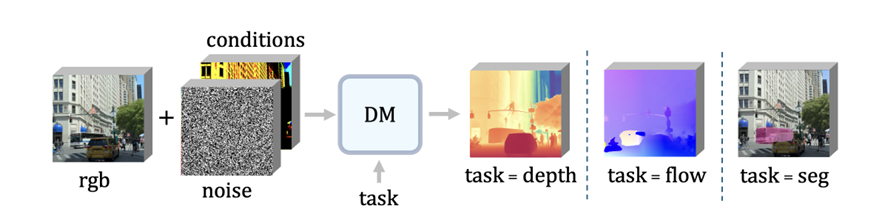
\includegraphics[width=0.5\linewidth]{figure1.png}
    \caption{\textbf{A Unified Framework}: We fine-tune a pre-trained Diffusion Model (DM), for visual
perception tasks. We take a RGB image, and a conditional image (i.e. next video frame, occlusion
mask, etc.), along with the noised image of the ground truth prediction. Our model generates pre
dictions for visual tasks such as depth estimation, optical flow prediction, and amodal segmentation,
based on the conditional task embedding. We train a generalist model that can perform all three
tasks with exceptional performance.}
    \label{fig:framework}
\end{figure}

\section{Related Work}
    \paragraph{Generative Modeling: } The generative modeling literature spans several major families of methods:
VAEs \citep{kingma2013auto}, GANs \citep{goodfellow2014generative}, normalizing flows \citep{rezende2015variational},
autoregressive models \citep{vandenOord2016pixel}, and diffusion models \citep{sohl2015deep,ho2020denoising}. Among these, Denoising Diffusion Probabilistic Models (DDPMs) \citep{ho2020denoising}
have proven especially good at scaling for image and video generation. Well-known examples
include Latent Diffusion Models \citep{rombach2022high}, which gain efficiency by operating in a compressed
latent space rather than pixel space; Imagen \citep{saharia2022photorealistic}, which instead generates directly in
pixel space at progressively higher resolutions; and Consistency Models \citep{song2023consistency}, which target
faster sampling without sacrificing generation quality. More recent approaches such as Rectified Flow \citep{liu2022rectified} and Flow Matching \citep{lipman2023flow} borrow training objectives from optimal
transport theory to learn continuous vector fields between data and target distributions, sidestepping
the discrete-timestep formulation that standard diffusion relies on. Rectified Flow addresses training
instabilities through flow regularization, while Flow Matching enables efficient sampling with fewer
discretization artifacts, making both attractive alternatives to conventional diffusion. Outside of
diffusion, Parti \citep{yu2022scaling} and MARS \citep{he2024mars} have demonstrated strong autoregressive image
generation, and Muse \citep{chang2023muse} introduced a transformer-based masked-image-generation approach.

\paragraph{\textbf{Scaling Diffusion Models:}} Diffusion models have also displayed strong scaling behavior along the axes
of data, model size, and compute. Latent Diffusion Models \citep{rombach2022high} were among the first to
show that training on large web-scale datasets with a U-Net backbone yields high-quality image
generation. DiT \citep{peebles2023scalable} instead swapped in a transformer backbone, revealing favorable scaling
properties for class-conditional generation. Building on this, Li et al.\ \citep{li2024scalability} examined alignment
scaling laws for text-to-image diffusion, and Fei et al.\ \citep{fei2024scalinga} pushed mixture-of-experts DiT models
up to 16B parameters while maintaining generation quality. A separate route to scaling transformers
is upcycling: Komatsuzaki et al.\ \citep{komatsuzaki2022sparse} showed that a dense transformer language model can
be converted into a mixture-of-experts model this way, without retraining from scratch. In a similar
spirit, EC-DiT \citep{sun2024ec} studies heterogeneous compute allocation for mixture-of-experts DiT
training, using expert-choice routing to adaptively assign compute to individual text-image samples.

\paragraph{\textbf{Diffusion Models for Perception Tasks: }}
 Beyond generation, diffusion models have been applied to a range of downstream
visual tasks, including depth estimation \citep{ji2023ddp,duan2023diffusiondepth,saxena2023monocular,saxena2024surprising,zhao2023unleashing}. Marigold \citep{ke2024repurposing} and GeoWizard \citep{fu2024geowizard}
are two more recent examples, both repurposing pre-trained diffusion models for monocular depth
estimation with strong results. With modest architectural changes, diffusion models have also been
applied to semantic segmentation over categorical
distributions \citep{hoogeboom2021argmax,brempong2022denoising,tan2022semantic,amit2021segdiff,baranchuk2021label,wolleb2022diffusion}, instance segmentation \citep{gu2024diffusioninst}, and panoptic
segmentation \citep{chen2023generalist}. Other applications include optical flow \citep{luo2024flowdiffuser,saxena2024surprising} and 3D understanding \citep{liu2023zero,jain2022zero,poole2022dreamfusion,wang2023score,watson2022novel}.

\section{Generative Pre-training}
We begin by studying how to scale diffusion pre-training efficiently. Our diffusion models are
trained for class-conditional image generation on a diffusion transformer (DiT) backbone, following
the original DiT training recipe \citep{peebles2023scalable}.

Starting with a target RGB image $I \in R^{u×u×3}$, where the resolution of the image is $u × u$, our
pretrained, frozen Stable Diffusion variational autoencoder \citep{rombach2022high} compresses the
target to a latent $z_0 \in R^{w× w× 4}$, where $w = u/8$. Gaussian noise is added at sampled time steps to obtain a noisy target latent. Noisy samples are generated as:
   \begin{equation}
       z_t=\sqrt{\alpha_t}\cdot z_0 + \sqrt{1-\alpha_t}\cdot\epsilon_t
   \end{equation}
for timestep $t$. The noise is distributed as 
$\epsilon \sim \mathcal{N}(0, I)$, $t \sim \text{Uniform}(T)$, 
with $T = 1000$ and
$\alpha_t := \prod_{s=1}^{t}(1 - \beta_s)$, 
with $\{\beta_1, \ldots, \beta_T\}$ as the variance schedule of a process.

In the denoising process, the class-conditional DiT $fθ(·)$, parameterized by learned parameters $θ$,
gradually removes noise from $z_t$ to obtain $z_{t−1}$. The parameters $θ$ are updated by noising $z_0$ with
sampled noise \epsilon at a random timestep $t$, computing the noise estimate, and optimizing the mean
squared loss between the generated noise and estimated noise in an $n$ batch size sample. We formally represent this as the following minimization problem:
 \begin{equation}
     \theta^{*}= arg\;min_\theta\;\mathcal{L}_\theta(z_t,\epsilon_i)=arg\;min_\theta \frac{1}{n}\sum _{i=1}^{n}(\epsilon_i-\hat{\epsilon_i})^2
 \end{equation}
where $θ^∗$ are the DiT learned parameters and \hat{\epsilon_i} is the DiT noise prediction for sample $i$.

   \subsection{Model Size}
   To study how pre-training scale affects performance, we train six dense DiT configurations of increasing size, summarized in Table~\ref{tab:dense_dit}, by varying both the number of transformer layers and the hidden dimension. All six are pre-trained on Imagenet-1K \citep{russakovsky2015imagenet} for 400k iterations, using a fixed learning rate of $1e-4$ and a batch size of 256. As Fig.~\ref{fig:fig2} shows, the bigger models consistently reach lower training loss, and the relationship follows a clean power law. Plotting train loss against compute (measured in MACs) yields the fitted relationship $L(C) = 0.23 \times C^{-0.0098}$. These pre-training results suggest that DiT scales gracefully even on a comparatively modest dataset, and this behavior carries over directly into stronger downstream performance after fine-tuning.
\begin{figure}[htbp]
\centering
    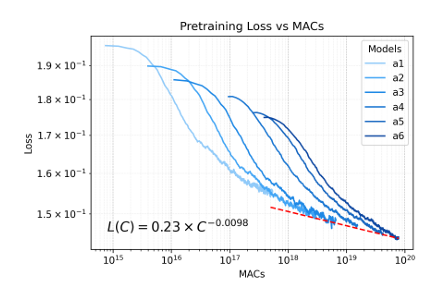
\includegraphics[width=.8\linewidth]{fig2.png}
    \caption{ \textbf{Scaling at Model Size:} For genera
tive pre-training of DiT models, we observe clear
power law scaling behavior as we increase the
model size.}
\label{fig:fig2}
\end{figure}

\subsection{Mixture of Experts}
Alongside the dense models, we pre-train Sparse Mixture-of-Experts (MoE) variants \citep{shazeer2017outrageously}, adopting the $S/2$
and $L/2$ configurations from \citep{fei2024scalingb}. Table~\ref{tab:moe_dit} lists the three MoE configurations we use,
which scale total parameter count by increasing hidden size, expert count, layer depth, and attention
heads. Every MoE block routes each token to its top-2 experts and additionally passes it through a
shared expert used by all tokens. We adopt the expert-balance loss
from \citep{fei2024scalingb} to keep load spread evenly across experts. This sparse
MoE recipe lets us grow parameter count while also improving throughput, making it more
compute-efficient than training a dense DiT model of comparable size. We train our DiT-MoE models
with the same training recipe as the dense DiT model using ImageNet-1K. Our approach enables
training DiT-MoE models to increase model capacity without increasing compute usage by another
order of magnitude, which would be required to train dense models of similar sizes.
\begin{table}[H]

\begin{minipage}[t]{0.48\textwidth}
\centering
\begin{tabular}{ccccc}
\toprule
     \textbf{model}&\textbf{params}&\textbf{dimension}&\textbf{head}&\textbf{layers}  \\
     \midrule
        a1 & 14.8M & 256  & 16 & 12 \\
        a2 & 77.2M & 512  & 16 & 16 \\
        a3 & 215M  & 768  & 16 & 20 \\
        a4 & 458M  & 1024 & 16 & 24 \\
        a5 & 1.2B  & 1536 & 16 & 28 \\
        a6 & 1.9B  & 1792 & 16 & 32 \\
    \bottomrule
\end{tabular}
\caption{\textbf{Dense DiT Models:} We scale dense DiT model size by increasing hidden dimension and number of layers linearly while keeping number of heads constant following \citep{yang2022tensor}.}
\label{tab:dense_dit}
\end{minipage}
\hfill 
\begin{minipage}[t]{0.48\textwidth}
\centering
\begin{tabular}{ccccc}
\toprule
\textbf{Model} & \textbf{Active / Total} & \textbf{Dim} & \textbf{Heads} & \textbf{Layers} \\
\midrule
S/2-8E2A  & 71M / 199M  & 384  & 6  & 12 \\
S/2-16E2A & 71M / 369M  & 384  & 6  & 12 \\
L/2-8E2A  & 1.0B / 2.8B & 1024 & 16 & 24 \\
\bottomrule
\end{tabular}
\caption{\textbf{MoE DiT Models:} We scale the MoE DiT models by increasing dimension size, number attention heads, layers, and experts following \citep{fei2024scalingb}.}
\label{tab:moe_dit}
\end{minipage}
\end{table}

\section{Fine-tuning for Perceptual Tasks}
This section looks at how to scale fine-tuning of the pre-trained DiT models to get the most out of
downstream perception performance. We adopt the image-to-image
diffusion training recipe from \citep{ke2024repurposing} and \citep{brooks2023instructpix2pix}, framing every
visual task as conditional denoising diffusion generation. Given an RGB image $I \in R_{u\times u\times3}$ and
its paired ground-truth image $D \in R_{u\times u\times3}$, we first project both into latent space, giving $i_0 \in R^{w\times w\times 4}$
and $d_0 \in R^{w\times w\times 4}$. Noise is added only to the ground-truth latent to produce $d_t$, which is then
concatenated with the RGB latent to form $z_t = \{i_0, d_t\}$. To accommodate the doubled number of
input channels, we modify the DiT model's first convolutional layer and halve its weight values, so that
predictions remain unchanged when the input is a plain RGB image, following \citep{ke2024repurposing}. Diffusion training then proceeds by denoising toward the ground-truth image. We run our fine-tuning compute-scaling ablations on the monocular depth estimation task, reporting Absolute Relative error and Delta1 error, and later carry the best configurations over to the other perceptual tasks.
\subsection{Effect of Model Size}
To study the effect of model size on fine-tuning, we take the pre-trained a1--a6 dense models
from Section~3.1 and fine-tune each on depth estimation. Fig.~\ref{fig:fig3} shows that the larger
DiT models reliably reach lower fine-tuning loss, again following a clear power law. Plotting both
training loss and validation metrics against compute (in MACs), we find that fine-tuned model
performance on both depth Absolute Relative error and depth Delta1 error follows the same power-law
pattern. These results give a strong signal for how performance should scale as fine-tuning compute
grows through model size alone.
\begin{figure}[htbp]
\centering
    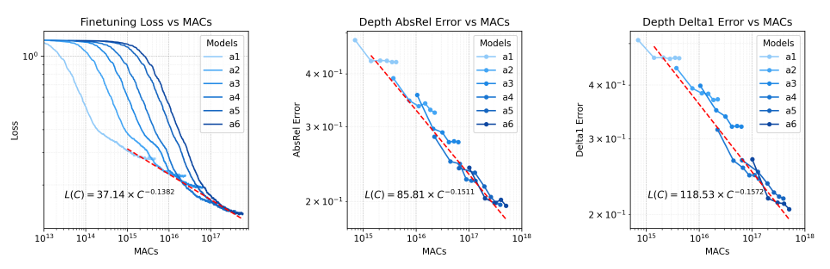
\includegraphics[width=.8\linewidth]{fig3.png}
    \caption{ \textbf{Effect of Model Size: }We fine-tune a1-a6 models on the Hypersim dataset for 30K
iterations with an exponential decay learning rate schedule from $3e-5$ to $3e-7$. We observe a strong
correlation between the fine-tuning loss scaling law and validation metric scaling laws.}
\label{fig:fig3}
\end{figure}
\subsection{Effect of Pre-training Compute}
We next examine how fine-tuning behaves as we vary the amount of pre-training given to the
DiT backbone. Four a4-configuration models are trained with different numbers of pre-training
steps while every other hyperparameter is held fixed, and each is then fine-tuned on the same
depth estimation dataset. Fig.~\ref{fig:fig4} shows that the depth estimation validation metrics follow a
power law as DiT pre-training steps increase, indicating that stronger pre-trained representations
translate into more effective use of fine-tuning compute.
\begin{figure}[htbp]
    \centering
    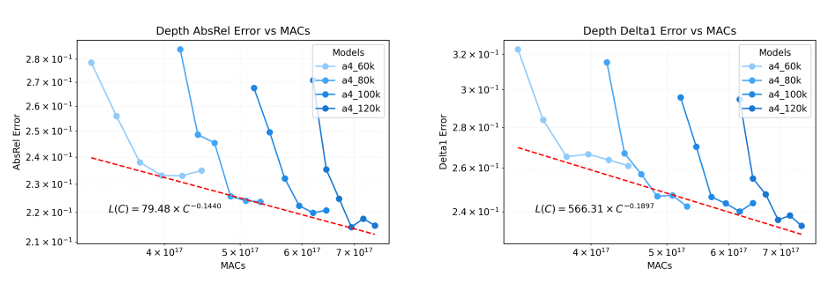
\includegraphics[width=0.8\linewidth]{fig4.png}
    \caption{\textbf{Effect of Scaling Model Pre-training Compute on Depth Estimation:} (a) Depth Abso
lute Relative Error vs. MACs. (b) Depth Delta1 Error vs. MACs. We pre-train four a4 models with
60K, 80K, 100K, and 120K steps. These models are then fine-tuned for 30K steps on the Hypersim
depth estimation dataset. We observe a clear power law as we increase the DiT pre-training compute
across depth estimation validation metrics.}
    \label{fig:fig4}
\end{figure}
\subsection{Effect of Image Resolution}
Image resolution is another lever on training compute, since a higher-resolution input produces
a longer token sequence for each forward pass. More tokens per image means more signal for the
model to learn from at training time, which can strengthen its internal representations and, in turn,
downstream performance. We take dense DiT-XL models pre-trained at $256\times256$ and $512\times512$
resolution from \citep{peebles2023scalable}, along with DiT-MoE L/2-8E2A models pre-trained at the same two
resolutions following \citep{fei2024scalingb}, and fine-tune each at its native resolution for depth estimation.
Figure~\ref{fig:fig5} shows that scaling fine-tuning compute this way, through image resolution, produces
meaningful gains in downstream depth estimation performance.
\begin{figure}[htbp]
    \centering
    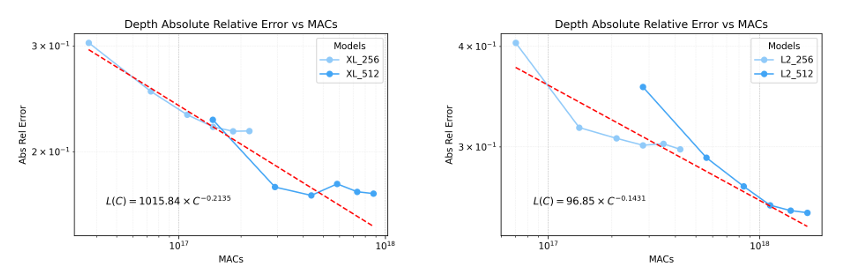
\includegraphics[width=0.8\linewidth]{fig5.png}
    \caption{\textbf{Effect of Image Resolution} We fine-tune DiT-XL and DiT-MoE L/2 models with resolutions of $256 \times 256$ and $512 \times 512$. We observe a power law when increasing image resolution
during training. By scaling the number of tokens per image by 4×, we achieve strong performance
on Depth Absolute Error, displaying the effect of increasing total dataset tokens for dense visual
perception tasks such as depth estimation.}
    \label{fig:fig5}
\end{figure}
\subsection{Effect of Upcycling}
While sparse MoE models offer an efficient way to grow model capacity, pre-training one from scratch is still costly. Sparse MoE Upcycling \citep{komatsuzaki2023sparse} offers a cheaper path: it turns a dense transformer checkpoint into an MoE model by duplicating each transformer block's MLP layer $E$ times (one per expert) and adding a learnable router that sends each token to its top-$k$ experts, whose outputs are then combined in a weighted sum at the end of the block. We apply upcycling to several dense DiT models that have already been fine-tuned for depth estimation, and continue fine-tuning the resulting upcycled models. Fig.~\ref{fig:fig6} shows the resulting scaling laws, with average gains of $5.3\%$ on Absolute Relative Error and $8.6\%$ on Delta1 error.

\begin{figure}[H]
    \centering
    
    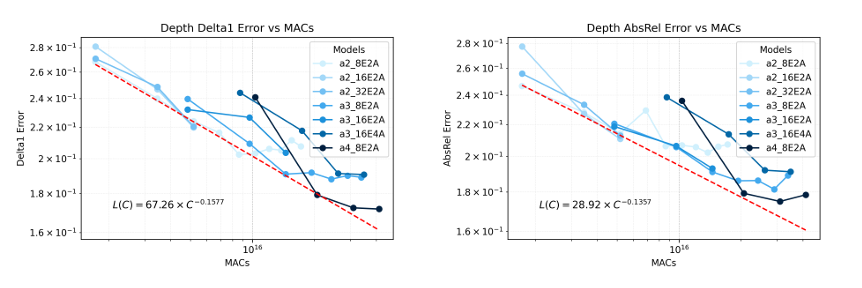
\includegraphics[width=\linewidth]{fig6.png} 
    
    \caption{\textbf{Effect of Upcycling.} We upcycle a2, a3, and a4 models fine-tuned for depth estimation with a varying number of total/active model experts. We continue fine-tuning each upcycled model for 15K iterations on the Hypersim depth estimation dataset. We observe a clear scaling law in the validation metrics as we increase fine-tuning compute with upcycling. The upcycled models can also achieve equivalent or superior performance to our dense a5 and a6 checkpoints, each of which utilize more compute during pre-training and fine-tuning. Increasing the total model experts and total active experts can also improve the downstream performance.}
    \label{fig:fig6}
\end{figure}
\section{Scaling Test-time Compute}
Scaling test-time compute is already a well-explored lever for autoregressive LLMs looking to improve long-horizon reasoning \citep{brown2024large, snell2024scaling, elrefai2024swag, openai2024reasoning}. Here, we show that the same lever reliably improves diffusion model performance on perceptual tasks. Fig.~\ref{fig:fig7} summarizes our overall approach: we first encode the input image into latent space with the Stable-Diffusion VAE \citep{rombach2022high}, then sample a target noise latent from a standard Gaussian and iteratively denoise it with DDIM \citep{song2021denoising} to obtain the final prediction.

\begin{figure}[htbp]
    \centering
    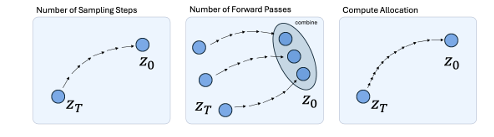
\includegraphics[width=\linewidth]{fig7.png}
    \caption{\textbf{Inference Scaling:} Diffusion models by design allow efficient scaling of test-time compute. First, we can simply increase the number of denoising steps to increase the compute spent at inference. Since we are estimating deterministic outputs, we can then initialize multiple noise latents and ensemble the predictions to get a better estimation. Finally, we can also reallocate our test-time compute budget for low and high frequency denoising by modifying the noise variance schedule.}
        \label{fig:fig7}
\end{figure}
\subsection{Effect of Scaling Inference Steps}
The simplest way to scale diffusion inference is to add more denoising steps. Because the model is trained to denoise across a range of timesteps, increasing the number of steps at test time naturally yields finer, more accurate predictions. This coarse-to-fine behavior, familiar from the generative setting, transfers directly to the discriminative case as well. Fig.~\ref{fig:fig8} shows that simply increasing the number of diffusion sampling steps, and thereby the total test-time compute, produces substantial gains in depth estimation performance.

\begin{figure}[htbp]
    \centering
    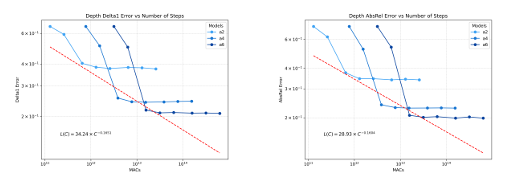
\includegraphics[width=\linewidth]{fig8.png}
    \caption{\textbf{Effect of Number of Sampling Steps.} (a) Delta1 Error vs. Number of Steps. (b) Absolute Relative Error vs. Number of Steps. For each model, we sample for $T \in [1, 2, 5, 10, 20, 50, 100]$ steps with the DDIM sampler. We show a clear power law scaling behavior in (a) and (b), displaying the effectiveness of scaling test-time compute by increasing the number of diffusion sampling steps.}
    \label{fig:fig8}
\end{figure}
\subsection{Effect of Test-time Ensembling}
Test-time ensembling offers a second way to scale inference compute, exploiting the fact that denoising different noise latents yields different downstream predictions. Here, we run $N$ forward passes per input sample and combine the outputs using one of two strategies. The first, naive ensembling, simply takes the pixel-wise median across all $N$ outputs. The second, following Marigold \citep{ke2024repurposing}, is median compilation, where we collect predictions $\{\hat{\boldsymbol{d}}_1, \dots, \hat{\boldsymbol{d}}_N\}$ that are affine-invariant, jointly estimate scale and shift parameters $\hat{s}_i$ and $\hat{t}_i$, and minimize the distances between each pair of scaled and shifted predictions $(\hat{\boldsymbol{d}}'_i, \hat{\boldsymbol{d}}'_j)$ where $\hat{\boldsymbol{d}}' = \hat{\boldsymbol{d}} \times \hat{s} + \hat{t}$. For each optimization step, we take the pixel-wise median $\boldsymbol{m}(x,y) = \text{median}(\hat{\boldsymbol{d}}'_1(x,y), \dots, \hat{\boldsymbol{d}}'_N(x,y))$ to compute the merged depth $\boldsymbol{m}$. Since it requires no ground truth, we scale ensembling by increasing $N$ to utilize more test-time compute. Fig.~\ref{fig:fig9} shows that this again produces a clear power-law improvement in depth estimation performance.

\begin{figure}[H]
    \centering
    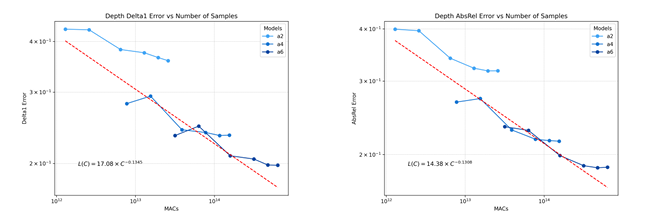
\includegraphics[width=\linewidth]{fig9.png}
    \caption{\textbf{Effect of Test Time Ensembling.} (a) Delta1 Error vs. Number of Forward Passes. (b) Absolute Relative Error vs. Number of Forward Passes. Ensembling multiple predictions from distinct noise initializations displays power law scaling behavior. We apply test-time ensembling values of $N \in [1, 2, 5, 10, 15, 20]$.}
    \label{fig:fig9}
\end{figure}
\subsection{Effect of Noise Variance Schedule}
A third way to scale test-time compute is to change where, rather than how much, compute is spent during denoising. Diffusion noise schedulers define how the variance of the added Gaussian noise evolves across the $T$ diffusion timesteps, and adjusting this schedule effectively reallocates compute toward earlier or later denoising steps. We compare three DDIM noise-level settings: linear, scaled linear, and cosine. The cosine schedule from \citep{nichol2021improved} decreases linearly starting from the midpoint of the corruption process, avoiding the overly aggressive early corruption seen with linear schedules. Fig.~\ref{fig:fig10} shows that, under a fixed compute budget, the cosine schedule outperforms linear schedules for DDIM on depth estimation.

\begin{figure}[htbp]
    \centering
    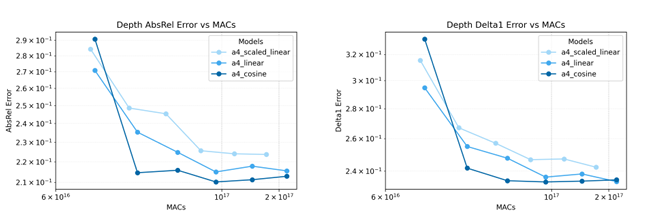
\includegraphics[width=\linewidth]{fig10.png}
    \caption{\textbf{Effect of Noise Variance (Beta) Schedule.} We fine-tune a4 models with three different beta schedules: linear, scaled linear, cosine. Reallocating compute with the cosine schedule to spend more time denoising at earlier timesteps significantly improved Delta1 and Absolute Relative Error rates.}
    \label{fig:fig10}
\end{figure}
\section{Putting It All Together}

Building on the lessons from our depth estimation scaling experiments, we extend our approach to train diffusion models for optical flow prediction and amodal segmentation. Across all three tasks, our efficient training and test-time compute-scaling strategies deliver substantial performance gains, matching or exceeding current state-of-the-art methods. These experiments offer practical guidance for applying diffusion models to visual perception under constrained compute. We then go a step further and train a single unified model capable of all three tasks at once, demonstrating that our scaling techniques generalize well beyond any one task. Altogether, our results show that these training and test-time scaling strategies remove the dependence on internet-scale pre-training data for high-quality visual perception with diffusion models. Fig.~\ref{fig:fig11} shows qualitative predictions from our models.

\subsection{Depth Estimation}

Combining what we learned from the depth estimation ablations, we assemble a model using the best training and inference settings identified so far. We fine-tune a DiT-XL model from \citep{peebles2023scalable} on Hypersim depth data for 30K steps, with a batch size of 1024, $512\times512$ resolution, and a learning rate that decays exponentially from $1.2e\text{-}4$ to $1.2e\text{-}6$. Inference uses median compilation ensembling with a cosine noise variance schedule, and, per our scaling experiments, 200 denoising steps with $N=5$ ensembled samples. Table~\ref{tab:depth_performance} shows the result: our model matches Marigold's validation performance on Hypersim and surpasses it on ETH3D, despite training on lower-resolution images with roughly \textbf{three orders of magnitude less pre-training data and compute}.

\begin{table}[htbp]
\centering
\begin{tabular}{lcccccccccc}
\toprule
\textbf{Method} & \multicolumn{2}{c}{\textbf{Hypersim}} & \multicolumn{2}{c}{\textbf{ETH3D}} & \multicolumn{2}{c}{\textbf{NYUv2}} & \multicolumn{2}{c}{\textbf{ScanNet}} & \multicolumn{2}{c}{\textbf{DIODE}} \\
& AbsRel $\downarrow$ & $\delta 1 \uparrow$ & AbsRel $\downarrow$ & $\delta 1 \uparrow$ & AbsRel $\downarrow$ & $\delta 1 \uparrow$ & AbsRel $\downarrow$ & $\delta 1 \uparrow$ & AbsRel $\downarrow$ & $\delta 1 \uparrow$ \\
\midrule
DiverseDepth & $-$   & $-$   & 22.8 & 69.4 & 11.7 & 87.5 & 10.9 & 88.2 & 37.6 & 63.1 \\
MiDaS        & $-$   & $-$   & 18.4 & 75.2 & 11.1 & 88.5 & 12.1 & 84.6 & 33.2 & 71.5 \\
LeReS        & $-$   & $-$   & 17.1 & 77.7 & 9.0  & 91.6 & 9.1  & 91.7 & 27.1 & 76.6 \\
Omnidata     & $-$   & $-$   & 16.6 & 77.8 & 7.4  & 94.5 & 7.5  & 93.6 & 33.9 & 74.2 \\
HDN          & $-$   & $-$   & 12.1 & 83.3 & 6.9  & 94.8 & 8.0  & 93.9 & 24.6 & 78.0 \\
DPT          & $-$   & $-$   & 7.8  & 94.6 & 9.8  & 90.3 & 8.2  & 93.4 & 18.2 & 75.8 \\
Marigold     & 13.5 & 87.5  & 6.5  & 96.0 & 5.5  & 96.4 & 6.4  & 95.1 & 30.8 & 77.3 \\
\midrule
\textbf{Ours}& \textbf{13.6} & \textbf{87.6} & \textbf{4.8} & \textbf{97.8} & \textbf{6.8} & \textbf{95.0} & \textbf{7.7} & \textbf{93.7} & \textbf{31.0} & \textbf{77.2} \\
\bottomrule
\end{tabular}
\caption{\textbf{Depth Estimation Performance Comparison on Multiple Datasets.} We achieve state-of-the-art performance on the ETH3D dataset and competitive performance across all other benchmarks. Notably, we closely match the performance of Marigold across all datasets with significantly less training compute.}
\label{tab:depth_performance}
\end{table}
\subsection{Optical Flow Prediction}

Optical flow estimation asks for the motion of objects between consecutive video frames, expressed as a dense, pixel-wise displacement field. We carry over essentially the same recipe used for depth estimation: a DiT-XL model trained on FlyingChairs for 40K steps, batch size 1024, $512\times512$ resolution, and a learning rate decaying exponentially from $1.2e\text{-}4$ to $1.2e\text{-}6$. Table~\ref{tab:optical_flow} compares our model against specialized optical flow methods.

\begin{table}[htbp]
  \centering
\begin{tabular}{lc}
\toprule
\textbf{Method} & \textbf{FlyingChairs EPE} $\downarrow$ \\
\midrule
DeepFlow & 3.53 \\
FlowNetS & 2.71 \\
FlowNetS+v & 2.86 \\
FlowNetS+ft & 3.04 \\
FlowNetS+ft+v & 3.03 \\
FlowNetC & 2.19 \\
FlowNetC+v & 2.61 \\
FlowNetC+ft & 2.27 \\
FlowNetC+ft+v & 2.67 \\
\midrule
\textbf{Ours (w/o ensembling)} & 3.45 \\
\textbf{Ours (w/ ensembling)} & 3.08 \\
\bottomrule
\end{tabular}
\caption{\textbf{Optical Flow Comparison with Specialized Techniques.} We evaluate our optical flow model on the FlyingChairs validation set. Our model achieves similar end-point error as specialized methods, including DeepFlow \citep{weinzaepfel2013deepflow} and FlowNet \citep{fischer2015flownet}. We train with significantly less data compared to other specialized methods, which use a several optical flow datasets. We generate predictions with and without test-time ensembling.}
\label{tab:optical_flow}
\end{table}




\subsection{Amodal Segmentation}

Amodal segmentation asks the model to infer the full shape and extent of an object, including parts hidden from view, which often demands higher-level scene reasoning for cluttered images. We fine-tune a DiT-XL model on the pix2gestalt dataset \citep{ozguroglu2024pix2gestalt} for 6K steps, using a batch size of 4096, $256\times256$ resolution, and the same exponentially decaying learning rate from $1.2e\text{-}4$ to $1.2e\text{-}6$. Table~\ref{tab:amodal_segmentation} compares our results against other methods.

\begin{table}[htbp]
\centering
\begin{tabular}{lccc}
\toprule
\textbf{Method} & \textbf{COCO-A} & \textbf{P2G} & \textbf{MP3D} \\
\midrule
PCNet & 81.35 & $-$ & $-$ \\
PCNet-Sup & 82.53 & $-$ & $-$ \\
SAM & 67.21 & $-$ & $-$ \\
SD-XL Inpainting & 76.52 & $-$ & $-$ \\
pix2gestalt & 82.9 & 88.7 & 61.5 \\
\midrule
\textbf{Ours} & 82.9 & 88.6 & 63.9 \\
\bottomrule
\end{tabular}
\caption{\textbf{Amodal Segmentation Performance (mIOU) Comparison Across Different Datasets.} This table compares mIOU performance across COCO-A, Pix2Gestalt, and MP3D datasets, showing the effectiveness of various methods. Our method is able to achieve competitive performance across all tasks, while training only on Pix2Gestalt.}
\label{tab:amodal_segmentation}
\end{table}

\subsection{One Model for All}

Finally, we train a single generalist DiT-XL model across all three tasks at once, using a mixed dataset that combines them. To let the model distinguish between task-specific embeddings during fine-tuning, we replace the standard patch embedding layer with a \texttt{PatchEmbedRouter} module, which routes each VAE embedding to the input convolutional layer appropriate for its task. Training otherwise mirrors our earlier recipes: $512\times512$ resolution images and a learning rate decaying exponentially from $1.2e\text{-}4$ to $1.2e\text{-}6$. We then upcycle the fine-tuned DiT-XL checkpoint into a DiT-XL-8E2A model and continue fine-tuning for a further 4K iterations. Fig.~\ref{fig:fig11} shows the resulting predictions, which highlight how well our scaling techniques generalize and transfer across different perception tasks.

   \begin{figure}[htbp]
       \centering
       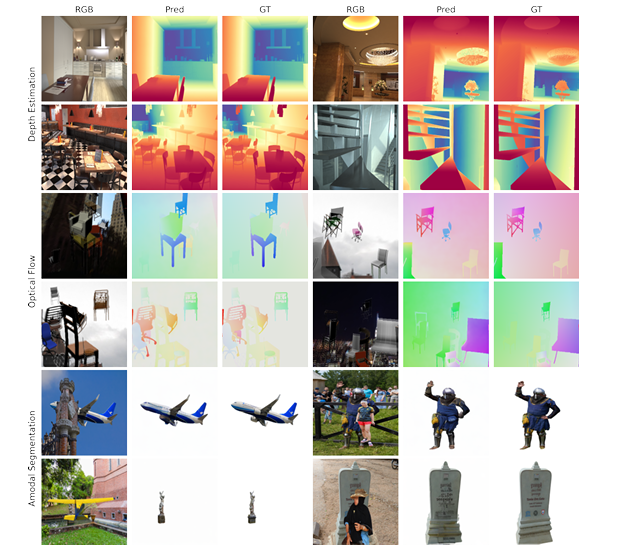
\includegraphics[width=0.8\linewidth]{fig11.png}
       \caption{\textbf{Depth Estimation, Optical Flow Estimation, and Amodal Segmentation Examples:}
Each row showcases results from our models for different tasks. (a) Depth estimation, with relative
scale and shift. (b) Optical flow, with scale and shift. (c) Amodal segmentation, where the model
sees an RGB image and segmentation of the occluded object; the task is to predict the amodal image}
       \label{fig:fig11}
   \end{figure}
\section{Conclusion}
This work examines how diffusion models scale for visual perception tasks. We explore several
routes to scaling diffusion training, including larger model size, mixture-of-experts architectures,
higher image resolution, and upcycling, and we show that test-time compute can also be scaled
efficiently by exploiting diffusion's iterative structure, yielding significant downstream gains.
Across the board, our experiments uncover consistent power laws for both training and inference
scaling. We hope these findings encourage further work on scaling both training and test-time
compute for iterative generative paradigms like diffusion, particularly for perception tasks.
\begin{thebibliography}{50}

\bibitem{amit2021segdiff}
Tomer Amit, Tal Shaharbany, Eliya Nachmani, and Lior Wolf.
\newblock Segdiff: Image segmentation with diffusion probabilistic models.
\newblock {\em arXiv preprint arXiv:2112.00390}, 2021.

\bibitem{baranchuk2021label}
Dmitry Baranchuk, Ivan Rubachev, Andrey Voynov, Valentin Khrulkov, and Artem Babenko.
\newblock Label efficient semantic segmentation with diffusion models.
\newblock {\em arXiv preprint arXiv:2112.03126}, 2021.

\bibitem{brempong2022denoising}
Emmanuel~Asiedu Brempong, Simon Kornblith, Ting Chen, Niki Parmar, Matthias Minderer, and Mohammad Norouzi.
\newblock Denoising pretraining for semantic segmentation.
\newblock In {\em Proceedings of the IEEE/CVF Conference on Computer Vision and Pattern Recognition}, pages 4175--4186, 2022.

\bibitem{brooks2023instructpix2pix}
Tim Brooks, Aleksander Holynski, and Alexei~A. Efros.
\newblock Instructpix2pix: Learning to follow image editing instructions.
\newblock {\em arXiv preprint arXiv:2211.09800}, 2023.

\bibitem{brown2024large}
Bradley Brown, Jordan Juravsky, Ryan Ehrlich, Ronald Clark, Quoc~V. Le, Christopher R{\'e}, and Azalia Mirhoseini.
\newblock Large language monkeys: Scaling inference compute with repeated sampling.
\newblock {\em arXiv preprint arXiv:2407.21787}, 2024.

\bibitem{chang2023muse}
Huiwen Chang, Han Zhang, Jarred Barber, AJ~Maschinot, Jose Lezama, Lu~Jiang, Ming-Hsuan Yang, Kevin Murphy, William~T. Freeman, Michael Rubinstein, Yuanzhen Li, and Dilip Krishnan.
\newblock Muse: Text-to-image generation via masked generative transformers.
\newblock {\em arXiv preprint arXiv:2301.00704}, 2023.

\bibitem{chen2023generalist}
Ting Chen, Lala Li, Saurabh Saxena, Geoffrey Hinton, and David~J. Fleet.
\newblock A generalist framework for panoptic segmentation of images and videos.
\newblock In {\em Proceedings of the IEEE/CVF International Conference on Computer Vision}, pages 909--919, 2023.

\bibitem{duan2023diffusiondepth}
Yiqun Duan, Xianda Guo, and Zheng Zhu.
\newblock Diffusiondepth: Diffusion denoising approach for monocular depth estimation.
\newblock {\em arXiv preprint arXiv:2303.05021}, 2023.

\bibitem{elrefai2024swag}
Karim El-Refai, Zeeshan Patel, Jonathan Pei, and Tianle Li.
\newblock Swag: Storytelling with action guidance, 2024.

\bibitem{fei2024scalinga}
Zhengcong Fei, Mingyuan Fan, Changqian Yu, Debang Li, and Junshi Huang.
\newblock Scaling diffusion transformers to 16 billion parameters.
\newblock {\em arXiv preprint arXiv:2407.11633}, 2024.

\bibitem{fei2024scalingb}
Zhengcong Fei, Mingyuan Fan, Changqian Yu, Debang Li, and Junshi Huang.
\newblock Scaling diffusion transformers to 16 billion parameters.
\newblock {\em arXiv preprint}, 2024.

\bibitem{fischer2015flownet}
Philipp Fischer, Alexey Dosovitskiy, Eddy Ilg, Philip H{\"a}usser, Caner Haz{\i}rba{\c{s}}, Vladimir Golkov, Patrick van~der Smagt, Daniel Cremers, and Thomas Brox.
\newblock Flownet: Learning optical flow with convolutional networks.
\newblock {\em arXiv preprint arXiv:1504.06852}, 2015.

\bibitem{fu2024geowizard}
Xiao Fu, Wei Yin, Mu~Hu, Kaixuan Wang, Yuexin Ma, Ping Tan, Shaojie Shen, Dahua Lin, and Xiaoxiao Long.
\newblock Geowizard: Unleashing the diffusion priors for 3d geometry estimation from a single image.
\newblock {\em arXiv preprint arXiv:2403.12013}, 2024.

\bibitem{goodfellow2014generative}
Ian Goodfellow, Jean Pouget-Abadie, Mehdi Mirza, Bing Xu, David Warde-Farley, Sherjil Ozair, Aaron Courville, and Yoshua Bengio.
\newblock Generative adversarial nets.
\newblock {\em Advances in Neural Information Processing Systems}, 27, 2014.

\bibitem{gu2024diffusioninst}
Zhangxuan Gu, Haoxing Chen, and Zhuoer Xu.
\newblock Diffusioninst: Diffusion model for instance segmentation.
\newblock In {\em IEEE International Conference on Acoustics, Speech and Signal Processing (ICASSP)}, pages 2730--2734, 2024.

\bibitem{he2024mars}
Wanggui He, Siming Fu, Mushui Liu, Xierui Wang, Wenyi Xiao, Fangxun Shu, Yi~Wang, Lei Zhang, Zhelun Yu, Haoyuan Li, Ziwei Huang, LeiLei Gan, and Hao Jiang.
\newblock Mars: Mixture of auto-regressive models for fine-grained text-to-image synthesis.
\newblock {\em arXiv preprint arXiv:2407.07614}, 2024.

\bibitem{ho2020denoising}
Jonathan Ho, Ajay Jain, and Pieter Abbeel.
\newblock Denoising diffusion probabilistic models.
\newblock {\em Advances in Neural Information Processing Systems}, 33:6840--6851, 2020.

\bibitem{hoogeboom2021argmax}
Emiel Hoogeboom, Didrik Nielsen, Priyank Jaini, Patrick Forr{\'e}, and Max Welling.
\newblock Argmax flows and multinomial diffusion: Learning categorical distributions.
\newblock {\em Advances in Neural Information Processing Systems}, 34:12454--12465, 2021.

\bibitem{jain2022zero}
Ajay Jain, Ben Mildenhall, Jonathan~T. Barron, Pieter Abbeel, and Ben Poole.
\newblock Zero-shot text-guided object generation with dream fields.
\newblock In {\em Proceedings of the IEEE/CVF Conference on Computer Vision and Pattern Recognition}, pages 867--876, 2022.

\bibitem{ji2023ddp}
Yuanfeng Ji, Zhe Chen, Enze Xie, Lanqing Hong, Xihui Liu, Zhaoqiang Liu, Tong Lu, Zhenguo Li, and Ping Luo.
\newblock Ddp: Diffusion model for dense visual prediction.
\newblock In {\em Proceedings of the IEEE/CVF International Conference on Computer Vision}, pages 21741--21752, 2023.

\bibitem{ke2024repurposing}
Bingxin Ke, Anton Obukhov, Shengyu Huang, Nando Metzger, Rodrigo~Caye Daudt, and Konrad Schindler.
\newblock Repurposing diffusion-based image generators for monocular depth estimation.
\newblock In {\em Proceedings of the IEEE/CVF Conference on Computer Vision and Pattern Recognition}, pages 9492--9502, 2024.

\bibitem{kingma2013auto}
Diederik~P. Kingma.
\newblock Auto-encoding variational bayes.
\newblock {\em arXiv preprint arXiv:1312.6114}, 2013.

\bibitem{komatsuzaki2022sparse}
Aran Komatsuzaki, Joan Puigcerver, James Lee-Thorp, Carlos~Riquelme Ruiz, Basil Mustafa, Joshua Ainslie, Yi~Tay, Mostafa Dehghani, and Neil Houlsby.
\newblock Sparse upcycling: Training mixture-of-experts from dense checkpoints.
\newblock {\em arXiv preprint arXiv:2212.05055}, 2022.

\bibitem{komatsuzaki2023sparse}
Aran Komatsuzaki, Joan Puigcerver, James Lee-Thorp, Carlos~Riquelme Ruiz, Basil Mustafa, Joshua Ainslie, Yi~Tay, Mostafa Dehghani, and Neil Houlsby.
\newblock Sparse upcycling: Training mixture-of-experts from dense checkpoints.
\newblock {\em arXiv preprint arXiv:2212.05055}, 2023.

\bibitem{li2024scalability}
Hao Li, Yang Zou, Ying Wang, Orchid Majumder, Yusheng Xie, R.~Manmatha, Ashwin Swaminathan, Zhuowen Tu, Stefano Ermon, and Stefano Soatto.
\newblock On the scalability of diffusion-based text-to-image generation.
\newblock In {\em Proceedings of the IEEE/CVF Conference on Computer Vision and Pattern Recognition}, pages 9400--9409, 2024.

\bibitem{lipman2023flow}
Yaron Lipman, Ricky~T.Q. Chen, Heli Ben-Hamu, Maximilian Nickel, and Matt Le.
\newblock Flow matching: Symmetrizing optimal transport and generative modeling.
\newblock {\em arXiv preprint arXiv:2301.13003}, 2023.

\bibitem{liu2023zero}
Ruoshi Liu, Rundi Wu, Basile Van~Hoorick, Pavel Tokmakov, Sergey Zakharov, and Carl Vondrick.
\newblock Zero-1-to-3: Zero-shot one image to 3d object.
\newblock In {\em Proceedings of the IEEE/CVF International Conference on Computer Vision}, pages 9298--9309, 2023.

\bibitem{liu2022rectified}
Xingchao Liu, Chengyue Gong, and Qiang Liu.
\newblock Rectified flow: A unified approach for free-form generative models.
\newblock {\em arXiv preprint arXiv:2209.07953}, 2022.

\bibitem{luo2024flowdiffuser}
Ao~Luo, Xin Li, Fan Yang, Jiangyu Liu, Haoqiang Fan, and Shuaicheng Liu.
\newblock Flowdiffuser: Advancing optical flow estimation with diffusion models.
\newblock In {\em Proceedings of the IEEE/CVF Conference on Computer Vision and Pattern Recognition}, pages 19167--19176, 2024.

\bibitem{nichol2021improved}
Alex Nichol and Prafulla Dhariwal.
\newblock Improved denoising diffusion probabilistic models.
\newblock {\em arXiv preprint arXiv:2102.09672}, 2021.

\bibitem{openai2024reasoning}
OpenAI.
\newblock Learning to reason with llms.
\newblock \url{https://openai.com/index/learning-to-reason-with-llms/}, September 2024.

\bibitem{ozguroglu2024pix2gestalt}
Ege Ozguroglu, Ruoshi Liu, D{\'\i}dac Sur{\'\i}s, Dian Chen, Achal Dave, Pavel Tokmakov, and Carl Vondrick.
\newblock pix2gestalt: Amodal segmentation by synthesizing wholes.
\newblock In {\em Proceedings of the IEEE/CVF Conference on Computer Vision and Pattern Recognition}, 2024.

\bibitem{peebles2023scalable}
William Peebles and Saining Xie.
\newblock Scalable diffusion models with transformers.
\newblock In {\em Proceedings of the IEEE/CVF International Conference on Computer Vision}, pages 4195--4205, 2023.

\bibitem{poole2022dreamfusion}
Ben Poole, Ajay Jain, Jonathan~T. Barron, and Ben Mildenhall.
\newblock Dreamfusion: Text-to-3d using 2d diffusion.
\newblock {\em arXiv preprint arXiv:2209.14988}, 2022.

\bibitem{rezende2015variational}
Danilo Rezende and Shakir Mohamed.
\newblock Variational inference with normalizing flows.
\newblock In {\em International Conference on Machine Learning}, pages 1530--1538. PMLR, 2015.

\bibitem{rombach2022high}
Robin Rombach, Andreas Blattmann, Dominik Lorenz, Patrick Esser, and Bj{\"o}rn Ommer.
\newblock High-resolution image synthesis with latent diffusion models.
\newblock In {\em Proceedings of the IEEE/CVF Conference on Computer Vision and Pattern Recognition}, pages 10684--10695, 2022.

\bibitem{russakovsky2015imagenet}
Olga Russakovsky, Jia Deng, Hao Su, Jonathan Krause, Sanjeev Satheesh, Sean Ma, Zhiheng Huang, Andrej Karpathy, Aditya Khosla, Michael Bernstein, Alexander~C. Berg, and Li~Fei-Fei.
\newblock Imagenet large scale visual recognition challenge.
\newblock {\em International Journal of Computer Vision}, 115(3):211--252, 2015.

\bibitem{saharia2022photorealistic}
Chitwan Saharia, William Chan, Saurabh Saxena, Lala Li, Jay Whang, Emily~L. Denton, Kamyar Ghasemipour, Raphael~Gontijo Lopes, Burcu~Karagol Ayan, Tim Salimans, et~al.
\newblock Photorealistic text-to-image diffusion models with deep language understanding.
\newblock {\em Advances in Neural Information Processing Systems}, 35:36479--36494, 2022.

\bibitem{saxena2023monocular}
Saurabh Saxena, Abhishek Kar, Mohammad Norouzi, and David~J. Fleet.
\newblock Monocular depth estimation using diffusion models.
\newblock {\em arXiv preprint arXiv:2302.14816}, 2023.

\bibitem{saxena2024surprising}
Saurabh Saxena, Charles Herrmann, Junhwa Hur, Abhishek Kar, Mohammad Norouzi, Deqing Sun, and David~J. Fleet.
\newblock The surprising effectiveness of diffusion models for optical flow and monocular depth estimation.
\newblock {\em Advances in Neural Information Processing Systems}, 36, 2024.

\bibitem{shazeer2017outrageously}
Noam Shazeer, Azalia Mirhoseini, Krzysztof Maziarz, Andy Davis, Quoc Le, Geoffrey Hinton, and Jeff Dean.
\newblock Outrageously large neural networks: The sparsely-gated mixture-of-experts layer.
\newblock {\em arXiv preprint arXiv:1701.06538}, 2017.

\bibitem{snell2024scaling}
Charlie Snell, Jaehoon Lee, Kelvin Xu, and Aviral Kumar.
\newblock Scaling llm test-time compute optimally can be more effective than scaling model parameters.
\newblock {\em arXiv preprint arXiv:2408.03314}, 2024.

\bibitem{sohl2015deep}
Jascha Sohl-Dickstein, Eric Weiss, Niru Maheswaranathan, and Surya Ganguli.
\newblock Deep unsupervised learning using nonequilibrium thermodynamics.
\newblock In {\em International Conference on Machine Learning}, pages 2256--2265. PMLR, 2015.

\bibitem{song2021denoising}
Jiaming Song, Chenlin Meng, and Stefano Ermon.
\newblock Denoising diffusion implicit models.
\newblock In {\em International Conference on Learning Representations}, 2021.

\bibitem{song2023consistency}
Yang Song, Prafulla Dhariwal, Mark Chen, and Ilya Sutskever.
\newblock Consistency models.
\newblock {\em arXiv preprint arXiv:2303.01469}, 2023.

\bibitem{sun2024ec}
Haotian Sun, Tao Lei, Bowen Zhang, Yanghao Li, Haoshuo Huang, Ruoming Pang, Bo~Dai, and Nan Du.
\newblock Ec-dit: Scaling diffusion transformers with adaptive expert-choice routing.
\newblock {\em arXiv preprint arXiv:2410.02098}, 2024.

\bibitem{tan2022semantic}
Haoru Tan, Sitong Wu, and Jimin Pi.
\newblock Semantic diffusion network for semantic segmentation.
\newblock {\em Advances in Neural Information Processing Systems}, 35:8702--8716, 2022.

\bibitem{touvron2023llama}
Hugo Touvron, Louis Martin, Kevin Stone, Peter Albert, Amjad Almahairi, Yasmine Babaei, Nikolay Bashlykov, Soumya Batra, Prajjwal Bhargava, Shruti Bhosale, et~al.
\newblock Llama 2: Open foundation and fine-tuned chat models.
\newblock {\em arXiv preprint arXiv:2307.09288}, 2023.

\bibitem{vandenOord2016pixel}
A{\"a}ron van~den Oord, Nal Kalchbrenner, and Koray Kavukcuoglu.
\newblock Pixel recurrent neural networks.
\newblock In {\em International Conference on Machine Learning}, pages 1747--1756. PMLR, 2016.

\bibitem{wang2023score}
Haochen Wang, Xiaodan Du, Jiahao Li, Raymond~A. Yeh, and Greg Shakhnarovich.
\newblock Score jacobian chaining: Lifting pretrained 2d diffusion models for 3d generation.
\newblock In {\em Proceedings of the IEEE/CVF Conference on Computer Vision and Pattern Recognition}, pages 12619--12629, 2023.

\bibitem{watson2022novel}
Daniel Watson, William Chan, Ricardo Martin-Brualla, Jonathan Ho, Andrea Tagliasacchi, and Mohammad Norouzi.
\newblock Novel view synthesis with diffusion models.
\newblock {\em arXiv preprint arXiv:2210.04628}, 2022.

\bibitem{weinzaepfel2013deepflow}
Philippe Weinzaepfel, Jerome Revaud, Zaid Harchaoui, and Cordelia Schmid.
\newblock Deepflow: Large displacement optical flow with deep matching.
\newblock In {\em Proceedings of the IEEE International Conference on Computer Vision}, pages 1385--1392, 2013.

\bibitem{wolleb2022diffusion}
Julia Wolleb, Robin Sandk{\"u}hler, Florentin Bieder, Philippe Valmaggia, and Philippe~C. Cattin.
\newblock Diffusion models for implicit image segmentation ensembles.
\newblock In {\em International Conference on Medical Imaging with Deep Learning}, pages 1336--1348. PMLR, 2022.

\bibitem{yang2022tensor}
Greg Yang, Edward~J. Hu, Igor Babuschkin, Szymon Sidor, Xiaodong Liu, David Farhi, Nick Ryder, Jakub Pachocki, Weizhu Chen, and Jianfeng Gao.
\newblock Tensor programs v: Tuning large neural networks via zero-shot hyperparameter transfer.
\newblock {\em arXiv preprint arXiv:2203.03466}, 2022.

\bibitem{yu2022scaling}
Jiahui Yu, Yuanzhong Xu, Jing~Yu Koh, Thang Luong, Gunjan Baid, Zirui Wang, Vijay Vasudevan, Alexander Ku, Yinfei Yang, Burcu~Karagol Ayan, et~al.
\newblock Scaling autoregressive models for content-rich text-to-image generation.
\newblock {\em arXiv preprint arXiv:2206.10789}, 2022.

\bibitem{zhao2023unleashing}
Wenliang Zhao, Yongming Rao, Zuyan Liu, Benlin Liu, Jie Zhou, and Jiwen Lu.
\newblock Unleashing text-to-image diffusion models for visual perception.
\newblock In {\em Proceedings of the IEEE/CVF International Conference on Computer Vision}, pages 5729--5739, 2023.

\end{thebibliography}
\end{document}